% Chapter Template

\chapter{Diseño e Implementación} % Main chapter title

\label{Chapter3} % Change X to a consecutive number; for referencing this chapter elsewhere, use \ref{ChapterX}

A continuación se describe el \textit{hardware} seleccionado para la extensión del circuito cargador, los criterios tomados en cuenta para su selección, el diseño del circuito y su conexión en \ref{sec:hard}. Luego se describe la arquitectura del sistema en \ref{sec:arq} y entra mas en detalle en \ref{sec:firm}, donde se describe el funcionamiento del \textit{firmware}. 

%----------------------------------------------------------------------------------------
%	SECTION 1
%----------------------------------------------------------------------------------------
\section{Hardware}
\label{sec:hard}

%-----------------------------------
%	SUBSECTION 1
%-----------------------------------
\subsection{El Panel Solar}
\label{subsec:panel} 
En el mercado existen distintas soluciones comerciales que se ajustan a las necesidades de cada aplicación. Ofrecen garantía limitada de entre 10 y 25 años y eficiencia de hasta 20 \% para módulos multicelda.
Es importante que los manufacturadores de módulos aseguren un control de calidad en las celdas fotovoltaicas. Estas están clasificadas según los defectos que puedan tener, identificadas con las letras A a la D. Celdas de grado A son aquellas que no presentan defectos visuales y cumplen con las especificaciones de los datos eléctricos \citep{grado}.

El sistema fotovoltaico propuesto originalmente esta basado en módulos con voltaje de 12V y 0.5A. Como medida de mitigación de riesgos, se planteó emplear componentes disponibles en el mercado local, y luego de tener en cuenta factores como grado de calidad (A), eficiencia, costos, tiempo de entrega, soporte pos-venta y al ser de Industria Argentina, se seleccionó el \textit{módulo fotovoltaico policristalino de alto rendimiento KS10T} \citep{solar} de la figura \ref{fig:ks10t} de SOLARTEC S.A. Se trata de paneles fabricados en base a celdas de silicio policristalino de alta eficiencia de conversión de energía (superior al 14\%).

Cuenta con certificado IRAM (Instituto Argentino de Normalización y Certificación), certificados CE (European Union: IEC61215 \textit{Photovoltaic Solar Testing Specifications} y IEC 61730 {\textit{Photovoltaic (PV) Module Safety Qualification}) y RoHs (\textit{DIRECTIVE 2002/95/EC: Restriction of Hazardous Substances}). Éste último le agrega ventaja frente a líderes del mercado internacional que no cumplen con la restricción de determinadas sustancias peligrosas. Sus características se muestran en la tabla \ref{tab:ks10t}. 
%y figura \ref{fig:mecanicas}\footnote{Fuente: SOLARTEC S.A. Todas las distancias están expresadas en mm.}.

La curva de la figura \ref{fig:curva}, muestra la corriente máxima de cortocircuito y la tensión máxima a circuito abierto del módulo \textit{KS10T}. Nótese que es capaz de entregar la tensión hasta exigir el máximo de corriente. Los valores y la curva están dados para condiciones de insolación de 1 KW/m2, masa atmosférica 1.5 y temperatura de celda de 25 \grados C\citep{solar}.

\vspace{10px}
 \begin{figure}[h!]
	\centering
    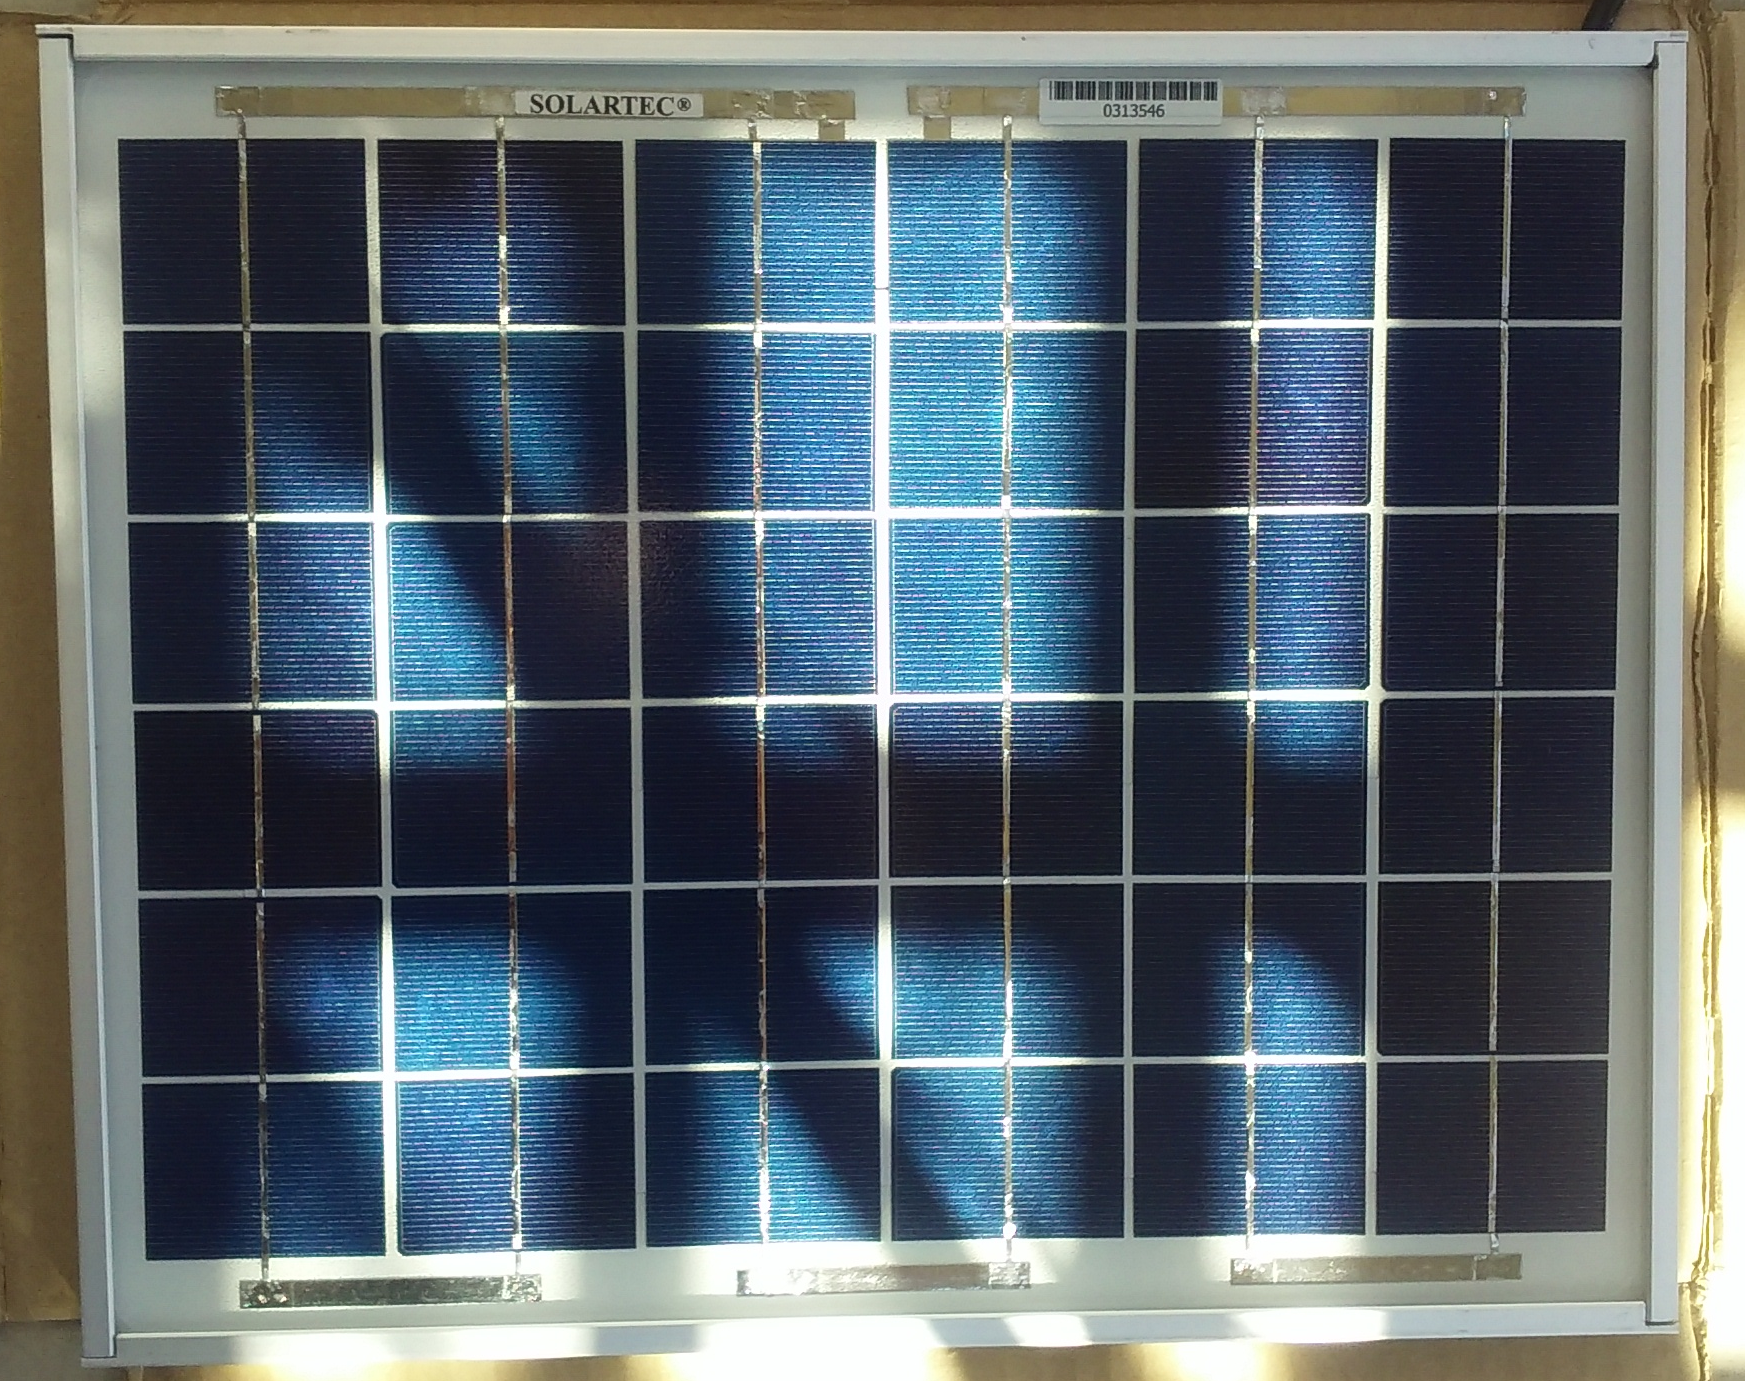
\includegraphics[width=0.6\textwidth]{./Figures/panel.png}
    	\caption{Módulo Fotovoltaico policristalino de alto rendimiento KS10T.}
	\label{fig:ks10t}
\end{figure}

\vspace{30px}
\begin{table}[ht]
	\centering
	\caption{Características del módulo fotovoltaico KS10T}
	\begin{tabular}{@{} l *2c @{}}    \toprule
		\emph{\textbf{Características}} & \emph{\textbf{Valor}} & \emph{\textbf{Unidad}}\\
		\midrule
		Potencia nominal	& 10 	& Wp	\\	
		Tensión a PN		& 17.4	& V\\
		Corriente a PN	& 0.58		& A\\
		Dimensiones		& 301x352x22 	& mm\\
		Peso				& 0.58		& Kg	\\
		\bottomrule
		\hline
	\end{tabular}
	\label{tab:ks10t}
\end{table}


%\begin{figure}[h]
%\centering
%\begin{subfigure}{.5\textwidth}
%%\begin{minipage}{\linewidth}
%  \centering
%    \includegraphics[width=0.5\textwidth]{./Figures/curva.JPG}
%  \caption[a)]{a)\protect\footnotemark}
%	\label{fig:curva}
%%\end{minipage}
%\end{subfigure}%
%\begin{subfigure}{.5\textwidth}
%  \centering
%    \includegraphics[width=0.5\textwidth]{./Figures/mecanicas.JPG}
%  	\caption[b)]{b)\protect\footnotemark}
%	\label{fig:mecanicas}
%\end{subfigure}
%\caption{a)Características eléctricas. b)Características mecánicas.}
%\label{fig:caract}
%\end{figure}

%\begin{figure}[h!]
%	\centering
%    \includegraphics[width=0.5\textwidth]{./Figures/mecanicas.JPG}
%    	\caption{Características mecánicas.}
%	\label{fig:mecanicas}
%\end{figure}

\vspace{30px}
\begin{figure}[h!]
	\centering
    \includegraphics[width=0.6\textwidth]{./Figures/curva.JPG}
    	\caption{Características eléctricas.}
	\label{fig:curva}
\end{figure}

%-----------------------------------
%	SUBSECTION 2
%-----------------------------------
\clearpage
\subsection{Circuito de Extensión Cargador}
\label{subsec:extensión}
Entre las interfaces para el usuario del nodo \textit{Mote LSE} esta el puerto USB, el cual alimenta al circuito de control de carga \textit{bq24080 1-A} con 5V(DC) a través de un conector USB micro-B. Este circuito es el empleado para la carga de la batería de Li-ion de 3.7V y 900mAh.

Es por esto que es necesario emplear una etapa reguladora de voltaje a la salida del panel, para la cual se utiliza el clásico regulador de Fairchild \textit{LM7805} de 1A \citep{7805}. Con unos pocos componentes (un condensador electrolítico como filtro a tierra para señales continuas para moderar la tensión eléctrica y las fluctuaciones de corriente y un condensador de poliéster para filtrar las señales espúreas de alta frecuencia, a la entrada y a la salida) entrega una salida de voltaje entre 4.75V y 5.25V. Además, ofrece protección contra sobrecarga térmica y cortocircuitos y opera entre -40 \grados C y +125 \grados C.

\vspace{30px}
\begin{figure}[h!]
	\centering
    \includegraphics[width=1\textwidth]{./Figures/circuito.jpg}
    	\caption{Diseño de Circuito de Extensión Cargador.}
	\label{fig:circuito}
\end{figure}

Un diseño de circuito alternativo, de montaje superficial, puede hacerse empleando el regulador \textit{TA78M05} de Toshiba Semiconductor. Ver la aplicación del circuito \textit{Current Boost Regulation} en \citep{78M05}.

%Para ver el diseño del PCB de la Extensión de Circuito Cargador, ver \ref{AppendixA}.

%-----------------------------------
%	SUBSECTION 3
%-----------------------------------
\subsection{Diagrama de Conexión}
\label{subsec:conexión}
El siguiente diagrama muestra la conexión entre la Circuito de Extensión Cargador 
(CEC) y el nodo \textit{Mote LSE}, así como la conexión entre el usuario y los nodos remotos. Para el detalle de la conexión del LPC-LINK y el mote, ver el Apéndice \ref{AppendixB}.

\vspace{30px}
\begin{figure}[h!]
	\centering
    \includegraphics[width=0.9\textwidth]{./Figures/conex.png}
    	\caption{Diagrama de Conexión.}
	\label{fig:conex}
\end{figure}

%----------------------------------------------------------------------------------------
%	SECTION 2
%----------------------------------------------------------------------------------------
\section{Arquitectura}
\label{sec:arq}
Cuando se diseña adecuadamente, los drivers de un dispositivo están abstraídos del hardware en sí, para que los usuarios finales, en este caso desarrolladores de software a nivel de aplicación, puedan controlar el hardware cuando una rutina en particular es llamada con el parámetro apropiado (API-CAPI \footnote{Application Programming Interface - Common Application Programming Interface}). Esto se refiere a la interfaz que las aplicaciones pueden usar para comunicarse directamente con el \textit{Mote LSE}.

Primero se usa la función del CMSIS, luego se define en código el handler de la excepción correspondiente, escribiendo en cada entrada del vector la dirección de memoria del handler asociado a la excepción.

A continuación se describe los niveles de abstracción de la arquitectura del firmware, desde los registros primitivos del hardware hasta la aplicación implementada, que incluye varios algoritmos que son usados para decidir de forma autónoma el modo de operación, si es necesario cargar la batería y generar alarmas de salud.

El modelo propuesto consiste en una arquitectura de capas (Ver figura \ref{fig:capas}). Los componentes de drivers de dispositivos que dan acceso a los diferentes recursos de hardware del \textit{Mote LSE} y sus funcionalidades están divididos en tres categorías. Los niveles de abstracción se describen en las siguientes capas:

\begin{figure}[h!]
	\centering
    \includegraphics[width=.5\textwidth]{./Figures/arq.png}
    	\caption{Modelo de Capas del Sistema.}
	\label{fig:capas}
\end{figure}

%-----------------------------------
%	SUBSECTION 1
%-----------------------------------
\subsection{Hardware}
\label{subsec:hardlayer} 

Esta capa contiene la libreria de Cortex ARM, \textit{Cortex Microcontroller Software Interface Standard} \citep{arm} (CMSISv2p00 LPC13xx) :Implementa las funciones de acceso al LPC1343.	

%-----------------------------------
%	SUBSECTION 1
%-----------------------------------
\subsection{HAL}
\label{subsec:hal} 

La capa de abstracción de hardware (en inglés, Hardware Abstraction Layer o HAL) implementa la portabilidad del sistema a otro \textit{hardware} distinto, siendo accesible en un único formato.

\noindent La HAL esta compuesta por:
\begin{itemize}
\item LPC1343 Drivers:
\begin{itemize}
	\item ssp.c : Implementa las interfaz entre el host y el cc2520.
	\item ssp.h : Contiene todas las macro que controlan la SPI.
	\item adc.c : Implementa las funciones de inicialización y lectura del ADC.
	\item adc.h : Contiene las macro que controlan el ADC.
	\end{itemize}
\item Board Drivers:
	\begin{itemize}
	\item cc2520.c : Implementa las funciones de acceso al transceiver cc2520.
	\item cc2520.h : Contiene todas las macro que controlan el pin CSn.
	\item ledpul.c : Implementa las funciones de acceso a los leds de la placa.
	\item ledpul.h : Contiene todas las macro que controlan los leds.
	\item bq.c : Implementa las funciones de lectura de estado y control del circuito controlador de carga bq24080.
	\item bq.h : Contiene todas las macro que controla los pines del bq24080.
	\end{itemize}
\item 802.15.4:
	\begin{itemize}
	\item cc2520-mac.c : Implementa las funciones de acceso al medio, arma el FCF e implementa los mecanismos de CSMA/CA.
	\item cc2520-mac.h : Define el tipo de datos necesarios para completar la trama (MHR, MAC Payload, MFR y PHR (Ver figura \ref{fig:data}) asignados en cc2520-task, mientras que el MFR (RSSI y CRC) y el SHR (secuencia de preámbulo y SFD) es implementado por el software embebido del transceiver cc2520 y completa la trama. Especifica el tipo de trama, el modo de direccionamiento MAC (short o extended: 16 o 64 bits) y la estructura de los octetos que forman el PSDU.
	\end{itemize}
\end{itemize}

\vspace{20px}
\begin{figure}[h!]
	\centering
    \includegraphics[width=1\textwidth]{./Figures/data.jpg}
    	\caption{Esquema del formato de la trama de Datos IEEE 802.15.4 \citep{802154}}
	\label{fig:data}
\end{figure}

%-----------------------------------
%	SUBSECTION 2
%-----------------------------------
\subsection{APPS}
\label{subsec:apps}
La capa APPS	o de aplicaciones esta compuesta por:
\begin{itemize}
\item cc2520Task:
	\begin{itemize}
	\item cc2520-task.c : Contiene la funcion framForming, que arma una trama de tipo DATA (formada con los parámetros relativos al 802.15.4 de cc2520-mac.c) y la guarda en el buffer de salida de cc2520. Los parámetros de entrada son la dirección de destino y el payload. Implementa las funciones de enviar y recibir datos.
	\item cc2520-task.h : Se incluyeron las funciones de operación referentes al transceiver (sendingData, waitingData)y la función FrameForming para ser utilizada por las capas de aplicación superiores, se define la variable MAXRETRIES que establece el máximo de retransmisiones de una trama y las variables de direccionamiento.
	\end{itemize}
\item monitoreoWsn:	
	\begin{itemize}
	\item main.c : Implementa las operaciones de medición referentes a cada modo de operación. Hace la lectura del ADC0 y ADC1 para la medición del voltaje de la batería y la temperatura ambiente respectivamente. Con la función frameForming de cc2520-task.c arma la trama con el payload que contiene todos las mediciones y estados de alarmas, y asigna la dirección del coordinador como dirección destino. Luego con la funcion ccTx del cc2520-mac, transmite el frame formado que esta contenido en el buffer de tx.
	\item include.h : Define el tipo de variables e incluye todos los \textit{header files} que utiliza de las demás capas de abstracción.
	\end{itemize}
\end{itemize}
%----------------------------------------------------------------------------------------
%	SECTION 3
%----------------------------------------------------------------------------------------
\section{Firmware}
\label{sec:firm}
El software embebido, llamado firmware en adelante, fue implementado en lenguaje de programación C y assembler. Éste implementa todas las funciones descriptas en la sección anterior.
 
Como punto de partida, se tomó el \textit{workspace} del Microstack 802.15.4 de la clase práctica de la asignatura Protocolos de Comunicación del Ing. Pablo Ridolfi y se realizaron las modificaciones en la libreria del Hardware y a nivel de HAL, para soportar el circuito controlador de carga bq24080 (Ver tabla \ref{tab:bq}) y el ADC, y así luego implementar las Apps sobre este Microstack.

\begin{table}[ht]
	\centering
	\caption{Asignación de puertos bq24080 - LPC1343}
	\begin{tabular}{@{} l *3c @{}}    \toprule
		\emph{\textbf{Puerto bq24080}} & \emph{\textbf{Puerto LPC1343}} & \emph{\textbf{PIN LPC1343}} & \emph{\textbf{PIN bq24080}}\\
		\midrule
		CE &  PIO3\_ 0 & 36 & 9	\\	
		PG	&  PIO3\_ 1 & 37 & 8\\
		STAT1 &  PIO1\_ 4 & 40 & 3\\
		STAT2 &  PIO2\_ 3 & 38 & 4\\
		\bottomrule
		\hline
	\end{tabular}
	\label{tab:bq}
\end{table}

%-----------------------------------
%	SUBSECTION 1
%-----------------------------------
\subsection{Descripción funcional}
\label{subsec:func} 
%Inter PAN 
%GPIO configurable al recibir un frame de determinadas características (puede esperar tramas de una serie de direcciones - frame filtering)
La función main() siempre es llamada cuando el programa se ejecuta por primera vez y de ahí se llama a las otras funciones.

Se define un ciclo de trabajo utilizando un contador decremental junto con el SysTick\_Handler para iniciar periódicamente la comunicación entre los nodos. Esto permite al diseñador escoger el fragmento de tiempo del ciclo activo para diferentes tipos de WSNs dependiendo del propósito de la aplicación, analizando la relación de compromiso entre la periodicidad del proceso de medición y el consumo de energía implicado.

La comunicación la inicia el dispositivo con la interrupción del SysTick\_Handler y espera la respuesta del coordinador, que se asume sin limitaciones de energía, por lo que luego de transmitir, vuelve al estado de recepción para monitorear a los demás dispositivos.

Los datos son transmitidos al nodo coordinador en una trama de datos 802.15.4, primero emplea la función ccFrameForming, que guarda los valores de las mediciones en el payload y asigna la dirección del coordinador como dirección destino, luego ccFrameTx guarda la trama formada en el buffer de salida.

Para cumplir con el requerimiento de almacenar en una memoria no volátil los estados de alarma y los parámetros monitoreados, éstos son almacenados en la memoria Flash del microcontrolador (la memoria SRAM necesita energía para que perduren los datos). 

\noindent La alarmas que reportan los dispositivos remotos son:
	\begin{itemize}
	\item TempAmbaja (1) : Reporta temperatura de ambiente baja.
	\item TempAmbalta (2) : Reporta temperatura de ambiente alta.
	\item ProyBatrest (3): En Modo Batería, el nodo hace un estimado experimental de la autonomía de la batería en base a la medición de su voltaje y le asigna un valor a un contador que se decrementa con cada interrupción del SysTickHandler. Esta alarma se activa cuando este contador llega a 0.
	\item TensionBat (4): Se activa cuando la tensión de la batería es menor a un valor prefijado.
	\end{itemize}
	
Estas alarmas son interpretadas por el nodo coordinador al hacer la lectura del primer byte del payload (MSB).(Ver tabla \ref{tab:edoalarm}). De la misma manera, el segundo byte (MSB) indica el modo de operación. (Ver tabla \ref{tab:edoope}).

\vspace{10px}
\begin{table}[ht]
	\centering
	\caption{Descripción del byte de Estado de Alarma}
	\begin{tabular}{@{} l *1c @{}}    \toprule
		\emph{\textbf{Valor}} & \emph{\textbf{Descripción}}\\
		\midrule
		00000000 & TempAmbaja\\	
		00000001 & TempAmbalta\\
		00000010 & ProyBatrest\\
		00000001 & TensionBat\\
		Otros & Reservado\\
		\bottomrule
		\hline
	\end{tabular}
	\label{tab:edoalarm}
\end{table}

\begin{table}[ht]
	\centering
	\caption{Descripción del byte de Estado de Operación}
	\begin{tabular}{@{} l *1c @{}}    \toprule
		\emph{\textbf{Valor}} & \emph{\textbf{Descripción}}\\
		\midrule
		00000000 &  Modo Batería\\
		11111111 &  Modo Panel\\
		Otros & Reservado\\
		\bottomrule
		\hline
	\end{tabular}
	\label{tab:edoope}
\end{table}

A nivel de la capa MAC, se implementa el modo de direccionamiento corto, de esta forma quedan 128 bytes disponibles para el payload. La siguiente tabla, muestra la estructura del payload de la trama que envía el dispositivo al coordinador. De la misma manera, el segundo byte (MSB) indica el modo de operación. (Ver tabla \ref{tab:dispcoor}).

\begin{table}[ht]
	\centering
	\caption{Descripción de la estructura del payload (Disp$\rightarrow$Coord)}
	\begin{tabular}{@{} l *6c @{}}    \toprule
		\emph{\textbf{Byte}} & \emph{\textbf{0}} & \emph{\textbf{1}} & \emph{\textbf{2}} & \emph{\textbf{3-4}} & \emph{\textbf{5}} & \emph{\textbf{6-127}}\\
		\midrule
		Significado & Edo. de & Edo. de & Temp. & Voltaje & Ciclos & Datos\\
		 & Alarma & Operación & Amb. & Bat. & de Carga & \\
		\bottomrule
		\hline
	\end{tabular}
	\label{tab:dispcoor}
\end{table}

Se implementan las funciones para reconocer el estado del circuito controlador de carga según el estado de los pines como indica la tabla \ref{tab:STAT}.

\begin{table}[ht]
	\centering
	\caption{Indicador de estado de los pines de estado del \textit{bq2480}}
	\begin{tabular}{@{} l *3c @{}}    \toprule
		\emph{\textbf{Estado}} & \emph{\textbf{STAT1}} & \emph{\textbf{STAT2}}\\
		\midrule
		Precarga en progreso &  ON & ON \\	
		%Carga rápida en progreso	&  ON & OFF \\
		Carga completa &  OFF & ON \\
		Modo sleep &  OFF & OFF \\
		\bottomrule
		\hline
	\end{tabular}
	\label{tab:STAT}
\end{table}

Un contador de cantidad de ciclos de carga se implementa con una variable que va aumentando cada vez que los estados de los pines STAT1 y STAT2 indican la carga completa de la batería y se desactiva el pin CE (\textit{Charge enable}) del \textit{bq24080}, el cual no es activado hasta que no alcance el límite de voltaje mínimo, controlando de esta manera la carga de la batería para preservar su vida útil. Mientras que el pin PG (\textit{Power good}) determina el modo de operación en función de su valor de entrada, que indica con un 0 (bajo) un voltaje de entrada válido, con lo cual establecerá el modo panel. 

VBATmon y la temperatura ambiente son medidas con el conversor AD0 y AD1 respectivamente (Ver Apéndice (Ver Apéndice \ref{AppendixB}). Para medir la temperatura se emplea el termistor lineal activo de baja potencia \textit{MCP9700} de Microchip \citep{termis}, con 1\grados C/bit de resolución para un ADC de 8-bit. Para obtener el voltaje de la batería se emplea la siguiente fórmula: \[V_{Bateria}=2xVBAT_{mon}\]

Los límites de temperatura de ambiente baja, alta y la tensión de batería baja son configurables en el firmware y pueden ser modificados por el coordinador cuando le envía una trama al dispositivo remoto. La siguiente tabla, muestra la estructura del payload de la trama que envía el coordinador al dispositivo (Ver tabla \ref{tab:coordisp}).

\begin{table}[ht]
	\centering
	\caption{Descripción de la estructura del payload (Coord$\rightarrow$Disp)}
	\begin{tabular}{@{} l *6c @{}}    \toprule
		\emph{\textbf{Byte}} & \emph{\textbf{0}} & \emph{\textbf{1}} & \emph{\textbf{2}} & \emph{\textbf{3}} & \emph{\textbf{4}} & \emph{\textbf{5-127}}\\
		\midrule
		Significado & Set & Ciclo & Límite & Límite & Límite & Datos\\
		 & Alarma & de Trabajo & Voltaje & Temp. Alta & Temp. Baja & \\
		\bottomrule
		\hline
	\end{tabular}
	\label{tab:coordisp}
\end{table}

Se optó por no hacer el sensado del consumo del circuito, primero porque no es posible realizar la medición de consumo de todos los componentes por el host, sino que los consumos pueden ser medidos en sus distintas etapas de operación (transmitiendo, recibiendo, modo sleep) con la ayuda de un instrumento externo (Ver capítulo \ref{Chapter4}) y segundo, porque comprometería aun mas la autonomía de un nodo de bajo consumo por transmitir información, si se quiere redundante, por ser determinista.

La autonomía del sistema permite que la WSN obtenga un conjunto de mediciones que es independiente del tiempo usado por servidores, pero también se podría implementar una interfaz a un servidor de tiempo para traducir el tiempo de la WSN a un tiempo común a los usuarios.

%Como premisa, modo sleep,
%\textit{wait for interrupt} buena practica
%%(_WFI)

%-----------------------------------
%	SUBSECTION 4
%-----------------------------------
\subsection{Diagramas de Topologías Implementadas}
\label{subsec:topo} 

Las topologías posibles de implementar son las siguientes:
\begin{figure}[h!]
	\centering
    \includegraphics[width=.8\textwidth]{./Figures/topologia.jpg}
    	\caption{Topología estrella y Peer-to-Peer.\citep{802154}}
	\label{fig:topo}
\end{figure}

En cuanto a la topología de árbol de cluster, no es posible su implementación, ya que la limitación de 4 nodos operativos disponibles no permite la configuración de una red de estas condiciones, por no cumplir con la densidad mínima de nodos (Ver figura \ref{fig:clust}). Los escenarios posibles, de tres nodos en una PAN y uno en otra, o dos nodos por PAN, no satisfacen los requerimientos. 

\begin{figure}[!htbp]
	\centering
    \includegraphics[width=.8\textwidth]{./Figures/cluster.jpg}
    	\caption{Topología árbol de cluster.\citep{802154}}
	\label{fig:clust}
\end{figure}

